\documentclass[10pt]{article}\usepackage[margin=.7in]{geometry}\usepackage{graphicx}\begin{document}\section*{Independent composed Add11 validity review}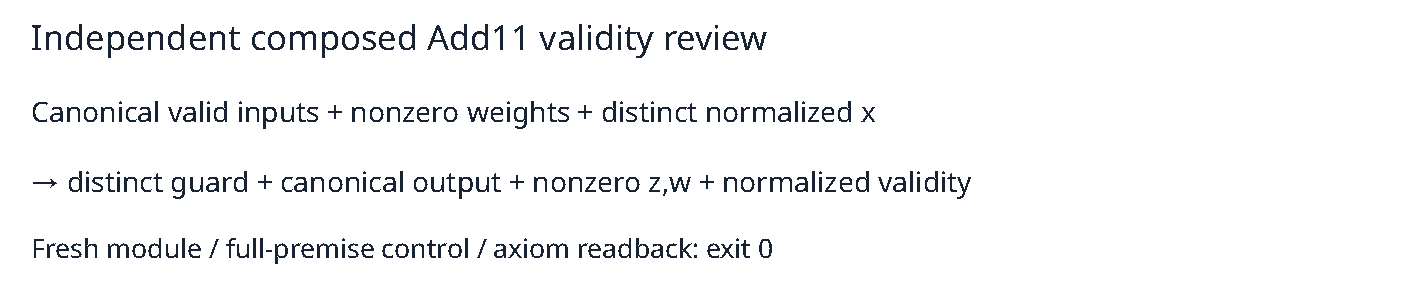
\includegraphics[width=\linewidth]{figure.pdf}
No blocking discrepancy was found. Producer hashes match. Fresh private theorem, controls and separate readback compiled with exit zero; only standard Lean axioms occur.

\paragraph{Composition} The theorem derives decoded nonzero weights from canonical nonzero words, uses exact payload decoding and field preservation, and rewrites all six decoded coordinates into the normalized output predicate. No output validity or coefficient equality is assumed. The conclusion includes the modeled distinct guard.

\paragraph{Control} The full nonunit-weight F7 fixture explicitly supplies both input divisibility witnesses and invokes the complete theorem. Equal-normalized-x and zero-weight boundaries are checked. Its polynomial $f=X^2$ is not presented as a smooth genus-two curve.

\paragraph{Scope} This establishes conditional branch-local literal-word validity. Compiler, counter, class-sum and whole-walk claims remain separate. Dependencies were reused and hash-bound, not rebuilt. REVIEW.md and receipts.json preserve details; producer failures remain retained. No scientific execution or repository edit occurred.
\end{document}